% !TeX root = ../defense.tex

\section{Implementation }
\frame{\sectionpage}

\begin{frame}{Linear Road}
    \begin{figure}
        \centering
        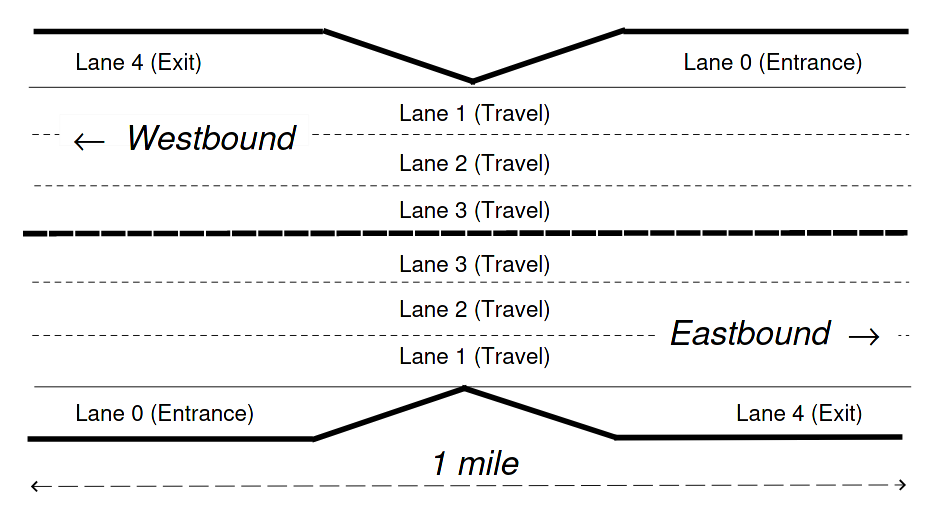
\includegraphics[scale=0.4]{lr.png}\\
        \caption{An Example Expressway Segment}
        \label{fig:lr_ex}
    \end{figure}
\end{frame}

\begin{frame}[fragile]{Linear Road: Query to execute}
    The goal is to execute the SegToll Query.
    \begin{lstlisting}[language=SQL, caption= SEGTOLL linear road query]
        SELECT car_id, exp_way, dir, seg
        FROM CarSegStr [PARTITION BY car_id ROWS 1], CurActiveCars
        WHERE CarSegStr.car_id = CurActiveCars.car_id;
        
        SELECT exp_way, dir, seg, AVG(speed) as speed,
        FROM CarSegStr [RANGE 5 MINUTES]
        GROUP BY exp_way, dir, seg;
        
        SELECT exp_way, dir, seg, COUNT(*) as volume
        FROM CurCarSeg
        GROUP BY exp_way, dir, seg;

        SELECT S.exp_way, S.dir, S.seg, basetoll*(V.volume-150)*(V.volume-150)
        FROM SegAvgSpeed as S, SegVol as V
        WHERE S.exp_way = V.exp_way and S.dir = V.dir and S.seg = V.seg
              and S.speed <= 40;
    \end{lstlisting}
\end{frame}

\begin{frame}{Implementation: Example of Query Plan}
$C_1=(S.exp\_way = V.exp\_way)$\\
$C_2=(S.dir = V.dir)$\\
$C_3=(S.seg = V.seg)$\\
$C_4=(S.speed <= 40)$\\
There are total of $4!=24$ possible orderings.\\
Few different query plans are
$$\pi_{\text{S.exp\_way, S.dir, S.seg, S.toll}}(\sigma_{C_1}(\sigma_{C_2}(\sigma_{C_3}(\sigma_{C_4}(\text{S,V})))))$$
$$\pi_{\text{S.exp\_way, S.dir, S.seg, S.toll}}(\sigma_{C_1}(\sigma_{C_2}(\sigma_{C_4}(\sigma_{C_3}(\text{S,V})))))$$
$$\pi_{\text{S.exp\_way, S.dir, S.seg, S.toll}}(\sigma_{C_1}(\sigma_{C_3}(\sigma_{C_2}(\sigma_{C_4}(\text{S,V})))))$$

\end{frame}

\begin{frame}{Implementation: Query Execution}
    \begin{enumerate}
        \item Mimicked the execution of query in C++.
        \item Given there are 24 possible orderings, executed all of them and recorded how much time and the number of operations they took.
        \item For each window of data store the column wise entropy and size of tables.
    \end{enumerate}
\end{frame}

\begin{frame}{Implementation: DQN}
    Training
    \begin{enumerate}
        \item Input the column wise entropy, the size of tables and ordering of operations.
        \item The reward for the training is taken to be the number of operations required.
    \end{enumerate}
    Prediction
    \begin{enumerate}
        \item Predict the reward for each ordering, for given entropy vector+ table size.\\
        \item The rewards represent number of operations required.
        \item Check which ordering has least number of operations, this ordering is optimal.
    \end{enumerate}
    Testing
    \begin{enumerate}
        \item Check if prediction for a test data point is same as the actual optimal ordering.
    \end{enumerate}
\end{frame}

\begin{frame}{Justification}
The things considered while determining the neural network to use for training the DQN are :-
    \begin{itemize}
        \item Value of loss function
        \item Time for prediction/ Complexity of model
        \item Resources for training
    \end{itemize}
\end{frame}

\begin{frame}{Justification}
    What we found was adding layers improves the accuracy of prediction of the optimal moves but not by significant margin.\\
    These are only query and data specific findings.
\end{frame}
